\begin{enumerate}
	\item Par lecture graphique, il semble que :
	\begin{itemize}
		\item la fonction $f$ est strictement croissante sur son ensemble de définition ;
		\item $\lim\limits_{x \to 2} f(x) = -\infty$, $\mathcal{C}_f$ semblant présenter une asymptote d'équation $x = 2$;
		\item $\lim\limits_{x \to +\infty} f(x) = +\infty$.
	\end{itemize}

	\item Résolvons l'équation sur $]2~;~+\infty[$ :

$\begin{aligned}
		f(x) = 0&\iff x\ln(x- 2) = 0\\
		& \iff x = 0 \text{ ou bien } \ln(x-2) = 0\quad \text{d'après la règle du produit nul}\\
		& \iff \ln(x-2) = 0\quad \text{car } x > 2\text{ donc } x\neq 0\\
		& \iff \exp\big(\ln(x-2)\big) = \exp(0)\quad \text{car exp est strictement croissante sur }\R\\
		& \iff x-2 = 1\\
		&\iff x = 3
\end{aligned}$

	L'équation a une unique solution : $x = 3$.

	\item On a : \quad $\begin{gathered}\lim\limits_{\substack{x \to 2\\x > 2}} x - 2 = 0^{+}\end{gathered}$\quad et donc, en posant $y = x - 2$, par composition, on en déduit :
	 $\begin{gathered}\lim\limits_{\substack{x \to 2\\x > 2}} \ln(x - 2) = \lim\limits_{\substack{y \to 0\\y > 0}} \ln(y) = -\infty\end{gathered}$.

Par ailleurs, \quad $\begin{gathered}\lim\limits_{\substack{x \to 2\\x > 2}} x = 2\end{gathered}$,\quad donc, par limite du produit : \quad $\begin{gathered}\lim\limits_{\substack{x \to 2\\x > 2}}[ x\times \ln(x-2)] = -\infty \end{gathered}$.

Cela confirme à la fois la conjecture sur la limite en 2 (en effet, comme $f$ n'est définie que sur $]2~;~+\infty]$, la limite en 2 est la limite à droite en 2), et cela confirme aussi la conjecture sur l'asymptote d'équation $x = 2$, qui est l'interprétation graphique de cette limite.

	\item Si\quad $u : x \longmapsto x - 2$\quad alors $u' : x \longmapsto 1$.

Ainsi \quad $x \longmapsto \ln(x-2)$ \quad est la composée $\ln \circ u$ et donc se dérive en :

$x \longmapsto \dfrac{u'(x)}{u(x)} = \dfrac{1}{x-2}$.

On dérive un produit de fonctions dérivables sur $]2~;~+\infty[$.

Pour tout réel strictement supérieur à 2, on a :

$f'(x) = 1 \times \ln(x - 2) + x \times \dfrac{1}{x - 2} = \ln(x-2) + \dfrac{x}{x - 2}$.

On arrive bien à l'expression annoncée pour $f'(x)$.

	\item \begin{enumerate}
		\item On a :\quad $\begin{aligned}[t]
			g'(x) &= f''(x) = \dfrac{1}{x - 2} + \dfrac{1 \times (x-2) - x \times 1}{(x-2)^2}\\
			&= \dfrac{1}{(x-2)} + \dfrac{-2}{(x-2)^2} = \dfrac{x-2}{(x-2)^2} + \dfrac{-2}{(x-2)^2}\\
			& = \dfrac{x - 4}{(x-2)^2}
		\end{aligned}$

On arrive bien à la forme demandée.

		\item $g'(x)$ est le quotient de $(x-4)$ par $(x-2)^2$.

Le dénominateur étant le carré d'un réel non nul, il est strictement positif, donc $g'(x)$ a le signe de $(x - 4)$. On peut donc établir le tableau de variations suivant :

\hfill~\begin{tikzpicture}
 			\tkzTabInit[lgt=4.5]
 			{$x$/0.7, signe de $x-4$/0.7,signe de $g'(x)$/0.7, variations de $g$/1.5}
 			{2,4,$+\infty$}
 			\tkzTabLine{,-,z,+,}
 			\tkzTabLine{d,-,z,+,}
 			\tkzTabVar{D+/$+\infty$ , -/$2 + \ln(2)$ , +/$+\infty$}
\end{tikzpicture}\hfill~

On a :\quad $g(4) = f'(4) = \ln(4 - 2) + \dfrac{4}{4 - 2} = \ln(2) + \dfrac{4}{2} = 2 + \ln (2)$.

		\item En observant le tableau de variations précédent, on a :

$2 > 1 \implies \ln(2) > 0$\quad donc on a $g(4) \geqslant 2 > 0$.

Donc, les variations de $g$ indiquent que $g$ atteint un minimum égal à $g(4) > 0$, pour $x = 4$.

On en déduit que la fonction $g$ est à valeurs strictement positives sur $]2~;~+\infty[$.

		\item Puisque $g$ est la fonction dérivée $f'$, on en déduit que $f'$ est à valeurs strictement positives sur $]2~;~+\infty[$, et donc que $f$ est strictement croissante sur $]2~;~+\infty[$.
	\end{enumerate}
\item On a établi les variations de $g = f'$ à la question \textbf{5. b.} :

\begin{itemize}
	\item sur $]2~;~4]$, $f'$ est décroissante, donc $f$ est concave;
	\item sur $[4~;~+\infty[$, $f'$ est croissante, donc $f$ est convexe.
\end{itemize}

$f$ change de convexité en $x = 4$, donc le point de coordonnées $\left(4~;~f(4)\right)$, est l'unique point d'inflexion de la courbe $\mathcal{C}_f$.

On a $f(4) = 4\times \ln(4 - 2) = 4\ln(2) = \ln \left(2^{4}\right) = \ln(16)$.

Les coordonnées exactes du point d'inflexion sont donc $(4~;~\ln(16))$.

	\item $\mathcal{C}_f$ admet une tangente de coefficient directeur égal à 3 au point d'abscisse $x$ si et seulement si $f'(x) = 3$, ou encore $g(x) = 3$.

On a $g(4) = 2 + \ln(2) \approx 2,7$. On a donc :

\begin{itemize}
		\item Sur $]2~;~4]$, $g$ est strictement décroissante, et continue (car dérivable), et 3 est une valeur strictement comprise entre $\lim\limits_{x \to 2} g(x)= +\infty$ et $g(4) = 2 + \ln(2) \approx 2,7$. D'après le corollaire du théorème des valeurs intermédiaires appliqué aux fonctions strictement monotones, il existe une unique solution à l'équation $g(x) = 3$ dans l'intervalle $]2~;~4]$, notée $\alpha$;
		\item De façon analogue, sur $]4~;~+\infty[$, $g$ est strictement croissante, et continue (car dérivable), et 3 est une valeur strictement comprise entre $\lim\limits_{x \to 4} g(x)\approx 2,7$ et $\lim\limits_{x \to +\infty} = + \infty$. Il existe aussi une unique solution à l'équation $g(x) = 3$ dans l'intervalle $]4~;~+\infty[]$, notée $\beta$ ;
\end{itemize}

Ainsi, l'équation $f'(x) = 3$ équivalente à $g(x) = 3$ admet exactement deux solutions $\alpha$ et $\beta$ sur $]2~;~+\infty[$.

Il y a donc exactement deux valeurs de $x$ ($\alpha$ et $\beta$) pour lesquelles la tangente à $\mathcal{C}_f$ a un coefficient directeur égal à 3.
\end{enumerate}
